\documentclass[article,final,14pt]{scrreprt}
\usepackage{cmap}
% \documentclass[14pt,pdf,hyperref={unicode}]{beamer}
\usepackage[utf8x]{inputenc}
\usepackage[russian]{babel}
\usepackage{amsfonts}
\usepackage{enumerate}
\usepackage{amsthm}
\usepackage{amssymb}
\usepackage{vmargin}
\usepackage{amsmath}
\usepackage{graphicx}
\usepackage{listings}
\usepackage{color}
\usepackage{multicol}
\usepackage{pb-diagram}
\usepackage[Bjornstrup]{fncychap}
\usepackage{fancyhdr}
\usepackage[svgnames,dvipsnames,x11names]{xcolor}
\usepackage{esint}
\usepackage{tocloft}
\usepackage{hyperref}
\usepackage{tikz}
\usepackage{epigraph}
\usepackage{setspace}
\usepackage{microtype}
\usepackage[dvipsnames]{xcolor}

\usetikzlibrary{calc}

\setpapersize{A4}
\setmarginsrb{2cm}{1.5cm}{1cm}{1.5cm}{0pt}{10mm}{0pt}{10mm}
\setlength{\parskip}{0.25cm}

\setlength\epigraphwidth{.5\textwidth}

% \usepackage[left=3.5cm,right=0cm,top=2cm,bottom=2cm]{geometry}

\usepackage{indentfirst}
\setlength{\parindent}{0.6cm}
% \sloppy

\DeclareGraphicsExtensions{.pdf,.png,.jpg}
\graphicspath{{ques/images/}}

\definecolor{linkcolor}{HTML}{610B0B}
\definecolor{urlcolor}{HTML}{6495ED}
\definecolor{lightgrey}{HTML}{9BABE7}
\definecolor{currentfancycolout}{HTML}{000000}

\hypersetup{pdfstartview=FitH,  linkcolor=linkcolor,urlcolor=urlcolor, colorlinks=true, pagecolor=linkcolor}

\setcounter{tocdepth}{2}
\linespread{1}

\fancyhead[RO]{\colorbox{currentfancycolout}{\color{white}{\textbf{\large \thepage}}}}  %% odd-right 
\fancyhead[LE]{\colorbox{currentfancycolout}{\color{white}{\textbf{\large \thepage}}}}  %%% even-left
\fancyhead[LO]{\colorbox{lightgrey}{\textbf{\thesection}}}% odd-left
\fancyhead[RE]{\colorbox{lightgrey}{\textbf{\thesection}}}% even-right 
\fancyhead[CE]{\rightmark}% odd-center, with the name of the Section
\fancyhead[CO]{\textsc{\leftmark}}% Even-center, with the name of the Chapter.
% \fancyfoot[L,R,C]{}

\makeatletter
\renewcommand*\env@matrix[1][*\c@MaxMatrixCols c]{%
  \hskip -\arraycolsep
  \let\@ifnextchar\new@ifnextchar
  \array{#1}}
\makeatother

\usepackage{enumitem}
% \setlist{noitemsep}
% \setlist[1]{\labelindent=\parindent} % < Usually a good idea
% \setlist[itemize]{leftmargin=*}
% \setlist[itemize,1]{label=$\triangleleft$}
% \setlist[enumerate]{labelsep=*, leftmargin=1.5pc}
% \setlist[enumerate,1]{label=\arabic*., ref=\arabic*}
% \setlist[enumerate,2]{label=\emph{\alph*}),
% ref=\theenumi.\emph{\alph*}}
% \setlist[enumerate,3]{label=\roman*), ref=\theenumii.\roman*}
% \setlist[description]{font=\sffamily\bfseries}

\begin{document}

\pagestyle{fancy}

% \fancyhf{} % очистили все колонтитулы
% \lhead{тратата} % левый верхний колонтитул
% \chead{} % центральный верхний
% \rhead{\textbf{\large \thepage}} % правый верхний
% \lfoot{} % левый нижний
% \cfoot{\textbf{\large \thepage}} % центральный нижний
% \rfoot{} % правый нижний

\renewcommand{\headrulewidth}{2pt} % линия под верхним к.
\renewcommand{\footrulewidth}{0pt} % линия над нижним к. 

\renewcommand\qedsymbol{$\blacksquare$}
\renewcommand\contentsname{Содержание}
\renewcommand\cftchapfont{\large\mdseries}

\newtheorem{theorem}{{\color{Purple} Теорема}}[chapter]
\newtheorem{problem}{Задача}
\newtheorem{lemma}{Лемма}[chapter]
\newtheorem{clair}{Утверждение}[chapter]

\theoremstyle{definition}
\newtheorem*{definition}{{\color{Purple} Определение}}[chapter]
\newtheorem{propose}{Предложение}[chapter]
\newtheorem{property}{Свойство}[chapter]
\newtheorem{condition}{Условие}[chapter]
\newtheorem{properties}{Свойства}[chapter]
\newtheorem*{conseq}{{\color{Purple}Следствие}}[chapter]
\newtheorem{remem}{Напоминание}[chapter]
\newtheorem{example}{Пример}[chapter]
\newtheorem{rulee}{Правило}[chapter]

\newtheorem*{question}{Вопрос}

\theoremstyle{definition}
\newtheorem*{remark}{{\color{Purple}Замечание}}

\newtheorem*{chck}{Проверка}
\newtheorem*{sign}{Обозначение}
\newtheorem*{uprazh}{Упражнение}

\newenvironment{Proof}       
	{\par\noindent{\bf Доказательство.}}
	{\hfill$\blacksquare$}
\newenvironment{solution}       
	{\par\noindent{\bf Решение.}}
	{\hfill$\blacksquare$}

\newcommand{\red}[1]{\textbf{\color{red}#1}}
\newcommand{\blue}[1]{\textbf{\color{blue}#1}}
\newcommand{\green}[1]{\textbf{\color{green}#1}}

\newcommand{\divisible}{\mathop{\raisebox{-2pt}{\vdots}}}

\newcommand{\RNumb}[1]{\uppercase\expandafter{\romannumeral #1\relax}}

\def\ton#1{1,2,\dots,#1}
\def\Set#1#2{\left\{#1\colon#2\right\}}
\def\MYdef{\mathrel{\stackrel{\rm def}=}}
\def\QUdef{\mathrel{\stackrel{\rm ?}=}}
\def\Ddef{\mathrel{\stackrel{\rm d}=}}
\def\PNdef{\mathrel{\stackrel{\rm \text{п.н.}}=}}

% \begin{center}
	{\Large \textbf{Как читать данный документ.}}
\end{center}

\noindent\Large{\textbf{Глава "1.Введение".}} 

В введении поясняется, с какой целью создан данный документ.\vspace{1cm}

\noindent\Large{\textbf{Глава "2.Цилиндрическая поверхность".}} 

В этой главе будут даны необходимые общие понятия о цилиндрических поверхностях.\vspace{1cm}

\noindent\Large{\textbf{Глава "3.Числовые характеристики."} }

Раздел описывает статистики, рассчитываемые для цилиндрических поверхностей, найденных в результате работы алгоритма, описанного в главе 2.\vspace{1cm}

\noindent\Large{\textbf{Глава "4.Рундист."} }

Дается определение рундиста на основе посчитанных статистик.\newpage


\tableofcontents
\chapter{Введение}

При оценке драгоценного камня одним из важнейших факторов является качество огранки. В связи с этим, чтобы уменьшить влияние текущих дефектов на стоимость камня, важной задачей является идентификация примитивов, аппроксимирующих различные части камня. \vspace{0.5cm}

В данном документе речь пойдет о \textit{рундисте}, части многогранника, аппроксимируемой цилиндрической поверхностью.

\begin{figure}[h!]
\center{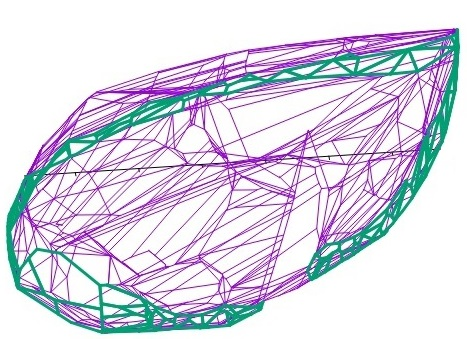
\includegraphics[scale=0.9]{Rundist.jpg}}
\end{figure}\newpage

\begin{center}
	\textbf{ \Large{Краткий обзор глав.}}
\end{center}

\noindent \textbf{ \large{Глава "1.Введение".}} 

В введении поясняется, с какой целью создан данный документ.\vspace{1cm}

\noindent\textbf{ \large{Глава "2.Цилиндрическая поверхность".}} 

В этой главе будут даны необходимые общие понятия о цилиндрических поверхностях.\vspace{1cm}

\noindent \textbf{ \large{Глава "3.Числовые характеристики".}} 

Раздел описывает статистики, рассчитываемые для цилиндрических поверхностей.\vspace{1cm}

\noindent \textbf{ \large{Глава "4.Рундист".}}

Дается определение рундиста на основе вычисленных статистик.\newpage
\chapter{Цилиндрическая поверхность.}

\begin{definition}[\textbf{Цилиндрическая поверхность.}]
	Поверхность Cyl называется {\color{Black} \textbf{цилиндрической}}, если она образована параллельным перемещением некоторой прямой $l$, называемой {\color{Black} \textbf{образующей}}, вдоль некоторой кривой $\gamma$, называемой {\color{Black} \textbf{направляющей}}.
\end{definition}

\begin{conseq}
	Векторы, перпендикулярные каждой точке цилиндрической поверхности ({\color{Black} \textbf{нормали поверхности}}), лежат в одной плоскости.
\end{conseq}

\begin{definition}
	$S^1 = \{ x \in \mathbb{R}^3: \; |x| = 1 \}$.
\end{definition}

\begin{conseq}
	Единичные нормали цилиндрической поверхности, выпущенные из $\vec{0}$, лежат на $C$. $C$ -- сечение $S^1$ некоторой плоскостью $\Pi$ через $\vec{0}$: $C_{big} = S^1 \cap \Pi$

	\vspace{1cm}
	\begin{figure}[h!]
	\center{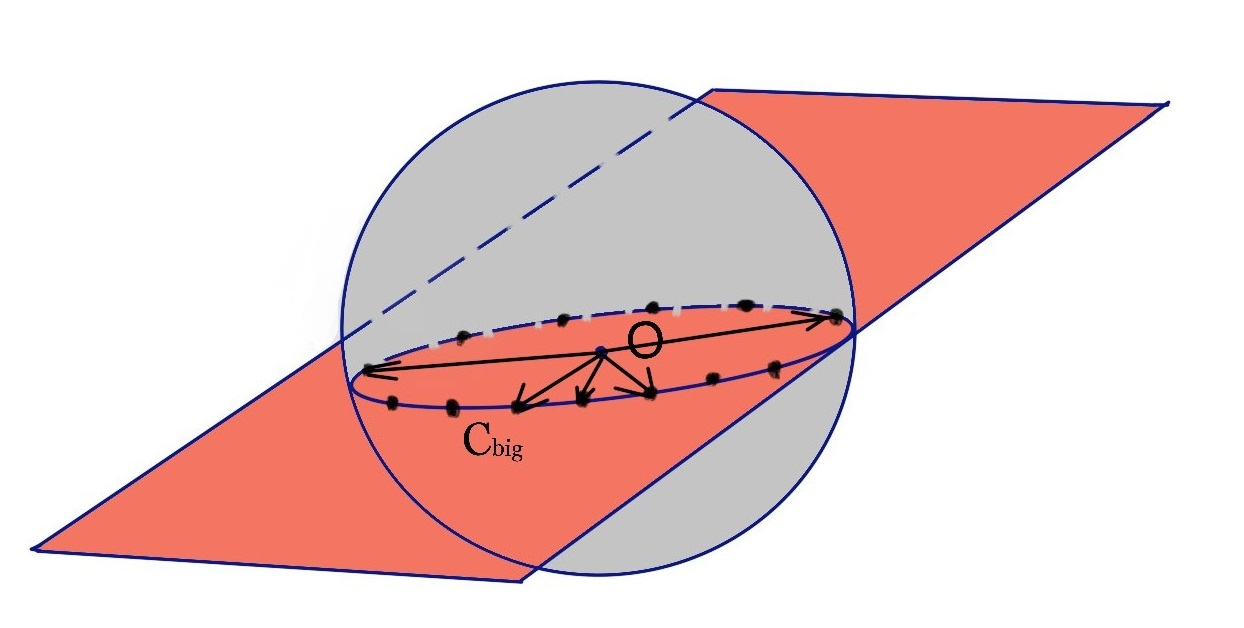
\includegraphics[scale=0.4]{1.jpg}}
	\end{figure}\vspace{0.5cm}
\end{conseq} \newpage

Рассмотрим множество единичных нормалей $\{ n_j \}_{j = 1}^N$ граней исходного многогранника P, выпущенных из $\vec{0}.$ 
Тогда для нахождения цилиндрических поверхностей на многограннике будем искать множества $N^{(i)} = \{ n_j \}_{j \in T_i}$, лежащие на C, где $T_i \subset \{ 1, \ldots, N\}$ -- набор индексов. Найденные наборы граней, соответствующие $N^{(i)}$, обозначим $\{ R_i\}$.

\begin{remark}
	$\vec{0}, \; N^{(j)}$ лежат на окружности C с некоторой погрешностью.
\end{remark}


\chapter{Числовые характеристики.}

\noindent$R = \{ Face_i \}_{i \in T}$ -- набор граней, соответствующий $\{ n_i\}_{i \in T}$.

\subsection*{\Large{Полоса набора $R$}.}

\begin{definition}[Аппроксимирующая плоскость.]
	$\Pi = \Pi(R)$ -- {\color{Black} \textbf{плоскость, аппроксимирующая вершины граней R}} в метрике 

	$$\begin{gathered}
			\rho(R, \; \Pi = \sum\limits_{i \in T}\sum\limits_{j_i}dist(v_{j_i}, \; \Pi(R)),
		\end{gathered}$$

	\noindentгде $dist(v_{j_i}, \; \Pi)$ -- евклидово расстояние от точки $v_{j_i}$ до плоскости $\Pi$, $\{ v_{j_i} \} $ -- вершины $Face_i$.

\end{definition}

\begin{remark}
	Далее, в качестве прямой, аппроксимирующей произвольный набор точек, будем использовать \textit{робастную линейную регрессию}.
\end{remark}

Развернем набор граней R на плоскости, перпендикулярной $\Pi$. 
\begin{figure}[h!]
\center{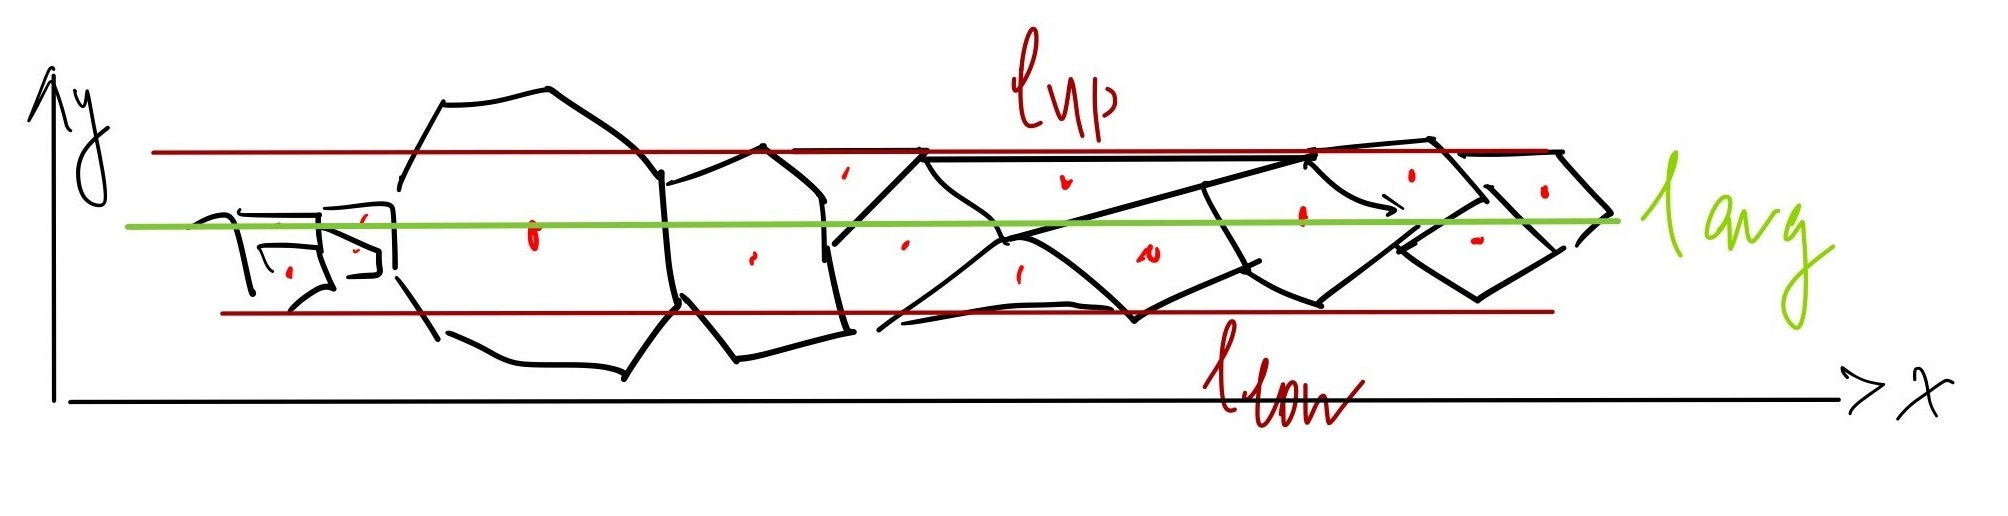
\includegraphics[scale=0.4]{Line.jpg}}
\caption{$\{ c_i\}$ -- красные точки.}
\end{figure}\newpage

Далее:
\begin{itemize}
	\item Приблизим центры граней $\{ c_i\}$ прямой $l_{avg}$.
	\item Найдем контур $Contour$ развернутого набора R.
	\item Рассмотрим вершины граней, лежащие выше прямой $l_{avg}$: $\{ v_k^{(u)}\} \in \cup_i Face_i: \; \forall \; k \; v_k^{(u)} \in Contour, \; y < v_k^{(u)}(y), \; (x, y) \in l_{avg}.$ Построим $l^{(up)}$ по набору  $\{ v_k^{(u)}\}$. Аналогично по точкам $\{ v_k^{(l)}\}$, лежащим ниже прямой $l_{avg}$, вычислим $l^{(low)}$.
\end{itemize}

\begin{definition}[Полоса рундиста ($girdle^{2D}$)]
	{\color{Black} \textbf{Полоса рундиста}} -- пространство плоскости, заключенное между $l^{(up)}$ и $l^{(low)}$ на участке $[x_{min}, x_{max}]$:
	$$\begin{gathered}
		girdle^{2D}(R):= \{ (x, y) \in \mathbb{R}^2: \; l^{(low)} \leq y \leq l^{(up)}\}.
	\end{gathered}$$
	\begin{figure}[h!]
	\center{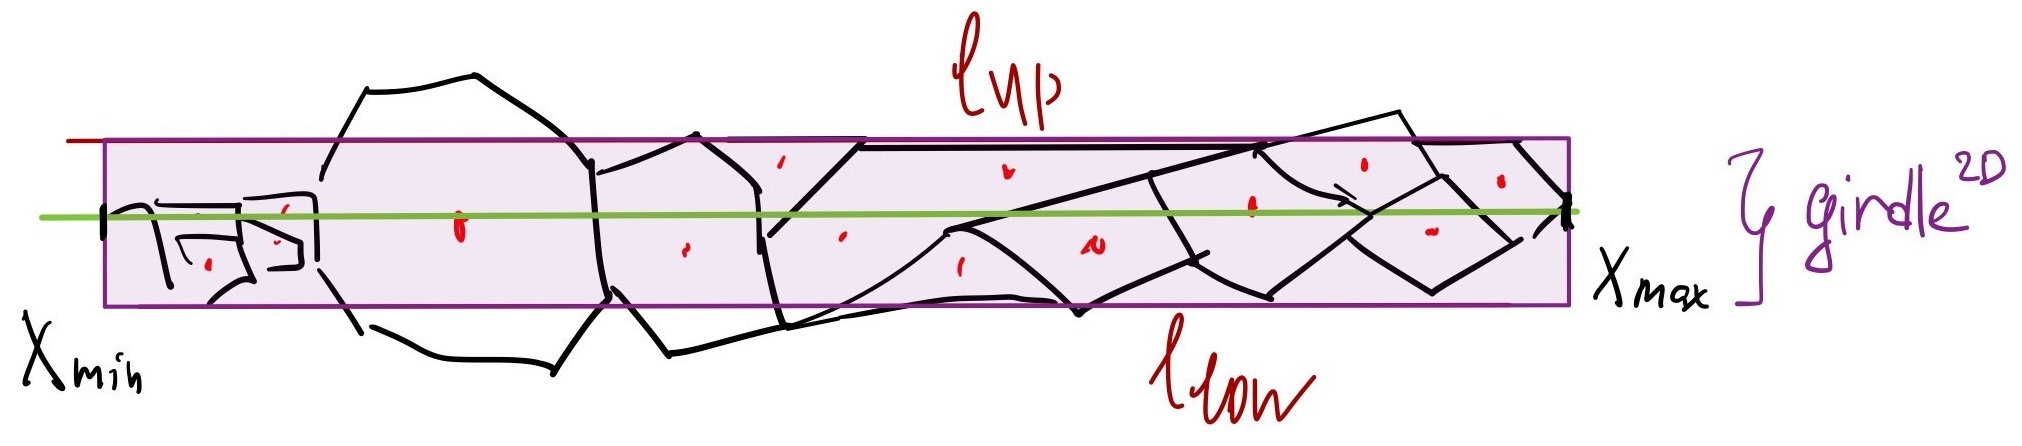
\includegraphics[scale=0.4]{Girdle.jpg}}
	\end{figure}

\end{definition}

\begin{definition}
	$x_{min} = \underset{x \in \{ v_k(x) \}}{argmin(x)}, \; x_{max} = \underset{x \in \{ v_k(x) \}}{argmax(x)}$.
\end{definition}

\begin{definition}[Размах полосы R (Amplitude).]
	$$\begin{gathered}
		Amplitude(R) := \underset{x \in [x_{min}, x_{max}]}{argmax}|l^{(up)}(x) - l^{(low)}(x)|,
	\end{gathered}$$
	где $l(x)$ -- координата $y$ точки $(x, y) \in l$.

	\begin{figure}[h!]
	\center{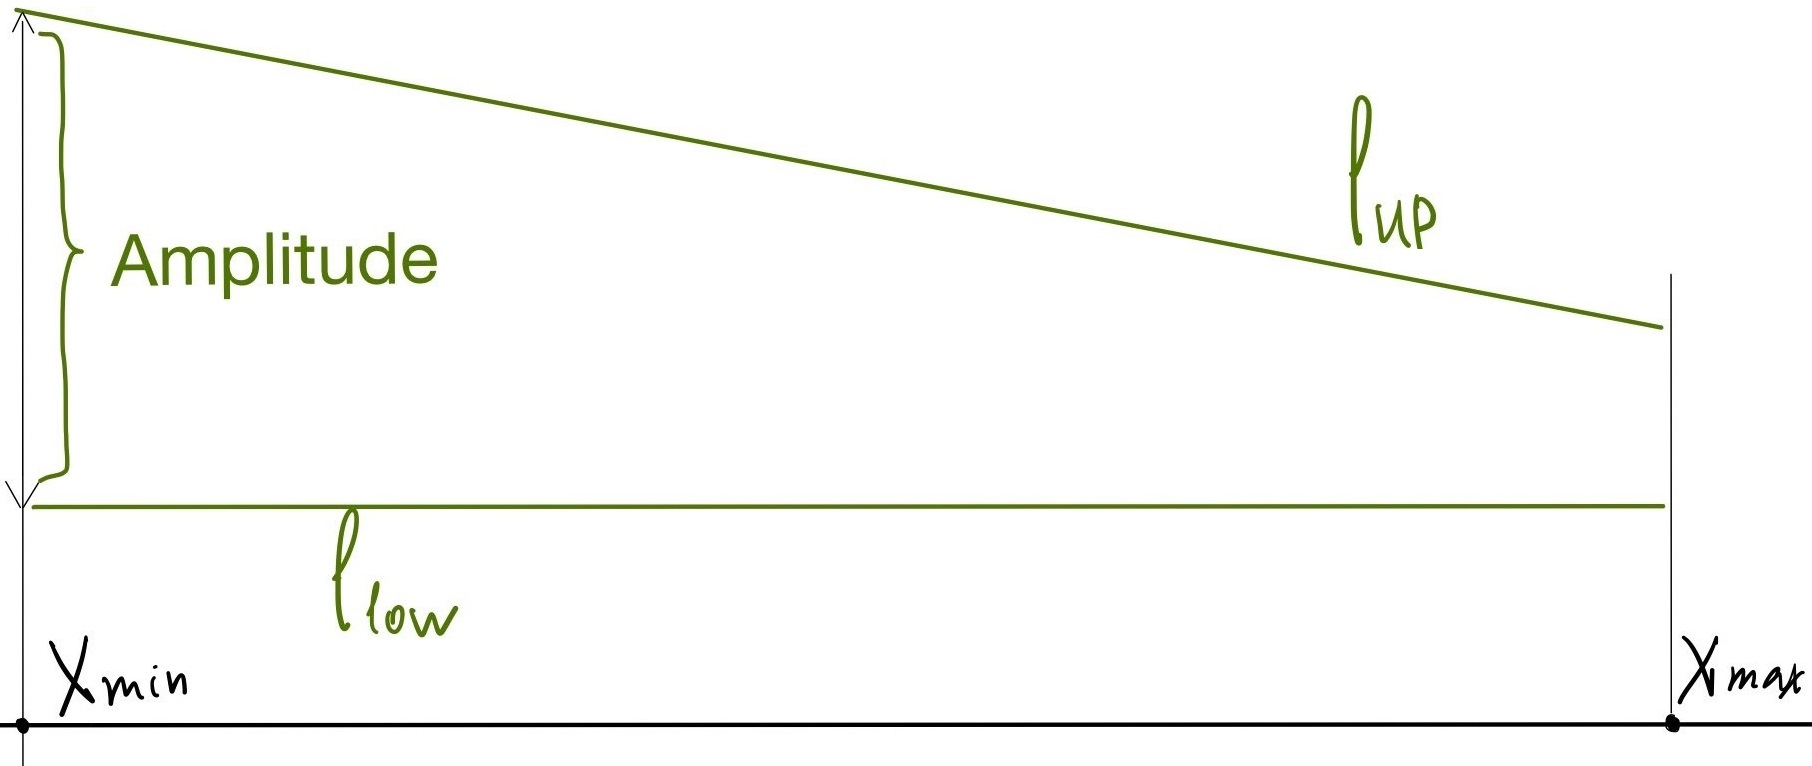
\includegraphics[scale=0.3]{Amplitude.jpg}}
	\end{figure}
\end{definition}\newpage

\begin{definition}[Параллельность $girdle^{2D}$]
	$$\begin{gathered}
		sin(R) := |sin \angle (l^{(up)}, l^{(low)})|.
	\end{gathered}$$

\end{definition}

\begin{definition}
	\noindentИзмерим, насколько сильно R выходит за свою полосу: посчитаем площадь частей граней $Face_i$, выходящих за полосу:

	$$\begin{gathered}
		S_{extern}(R) := \sum\limits_{i}Area(Face_i \cap \{ \mathbb{R}^2 \setminus girdle^{2D} \})
	\end{gathered}$$

	\begin{figure}[h!]
	\center{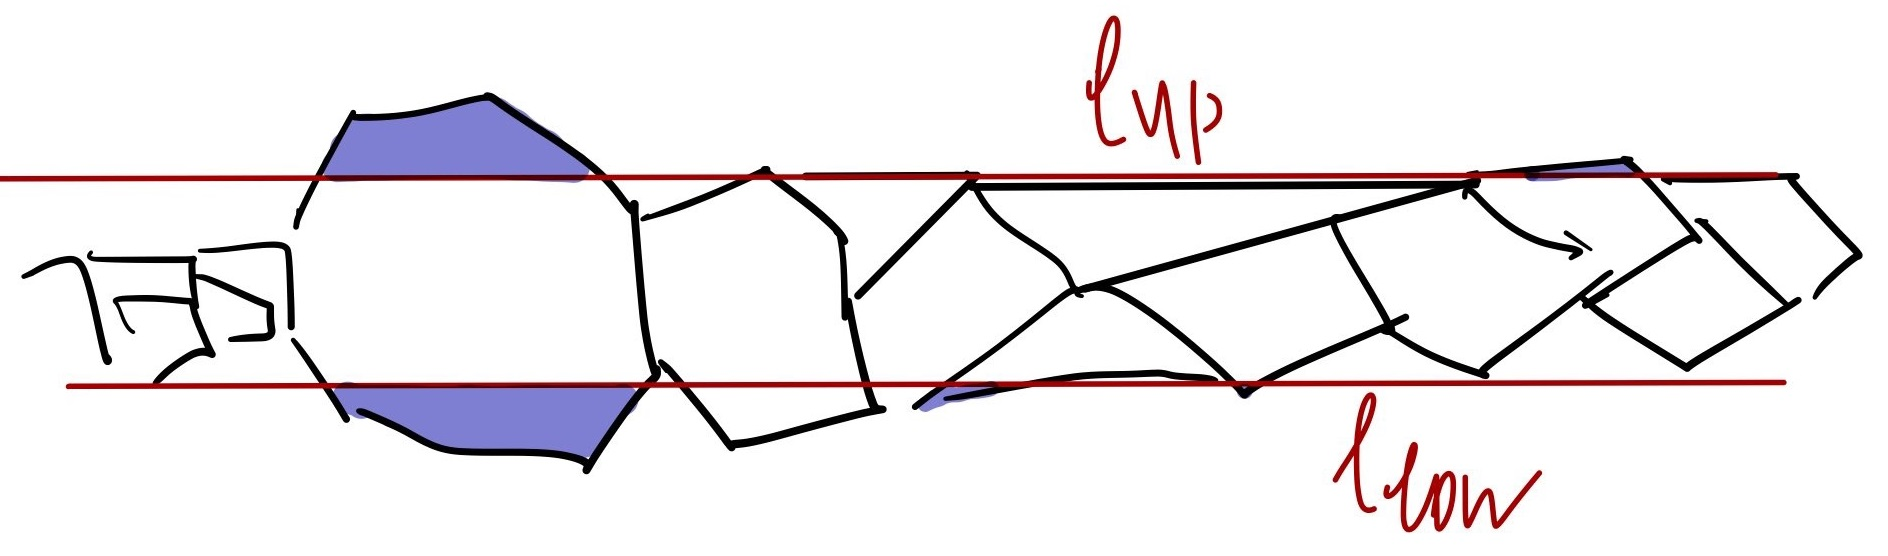
\includegraphics[scale=0.4]{Area_extern.jpg}}
	\caption{В примере на изображении выше находим суммарную площадь синих участков.}
	\end{figure}

\end{definition}

\begin{remark}
	\noindentВозможна ситуация, когда в R лежат наборы, не соответствующие (визуально) одной и той же части камня. Разобьем R на подмножества смежных граней: $R^i:\; \bigcup_i R^i = R.$ 

	\noindentОднако, может быть такое, что $\exists$ грани $\in R$, для которых среди элементов R нет смежных граней. 

	\noindentРассмотрим случай, когда такая грань $Face_{i_0}$ одна. Необходимо объединить ее с соответствующим ей набором $R^i$. Если $\exists $ вершина $v \in Face_{i_0}: \; v \in girdle^{2D}(R^i), $ то добавим $Face_{i_0}$ в $R^i$.

	\begin{figure}[h!]
	\center{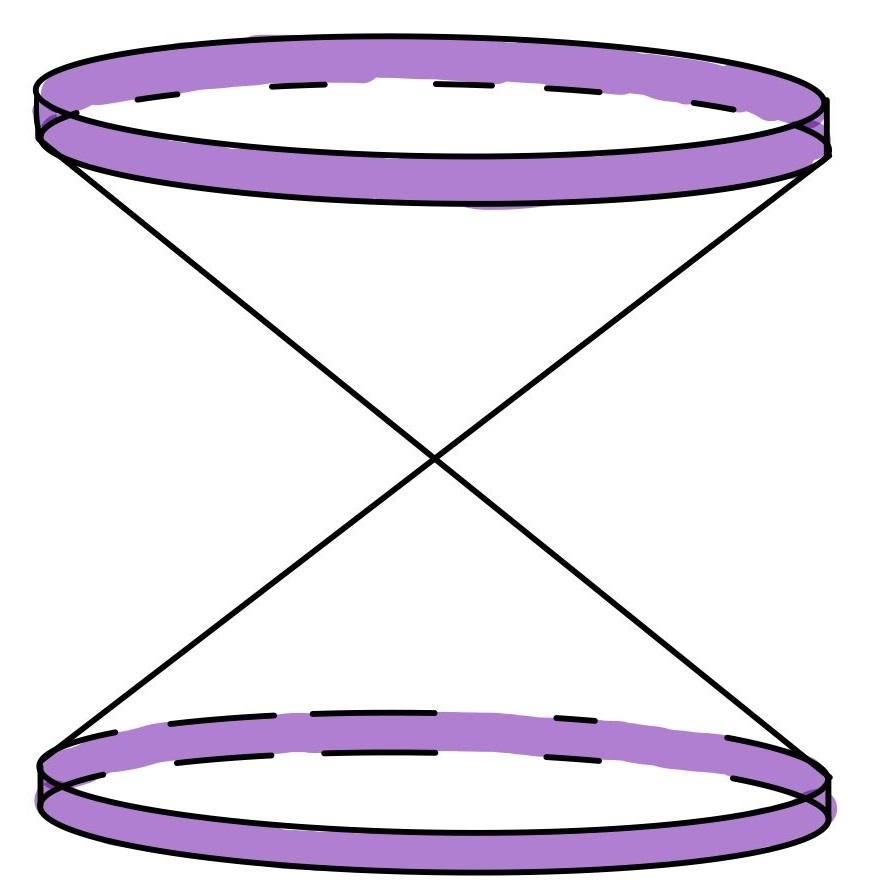
\includegraphics[scale=0.4]{TwoRund.jpg}}
	\caption{В примере на изображении выше фиолетовые части многогранника будут лежать в одном R.}
	\end{figure}\newpage
\end{remark}

\subsection*{\Large{Симметричность многогранника относительно набора $R$}.}

$\Pi$ делит $\mathbb{R}^3$ на два полупространства, $\Pi^+$ и $\Pi^-$, соответственно, делит многогранник P на $P^+ \in \Pi^+$ и $P^- \in \Pi^-$. Рассмотрим $P^+$, аналогично для $P^-$.\vspace{1cm}

\begin{figure}[h!]
\center{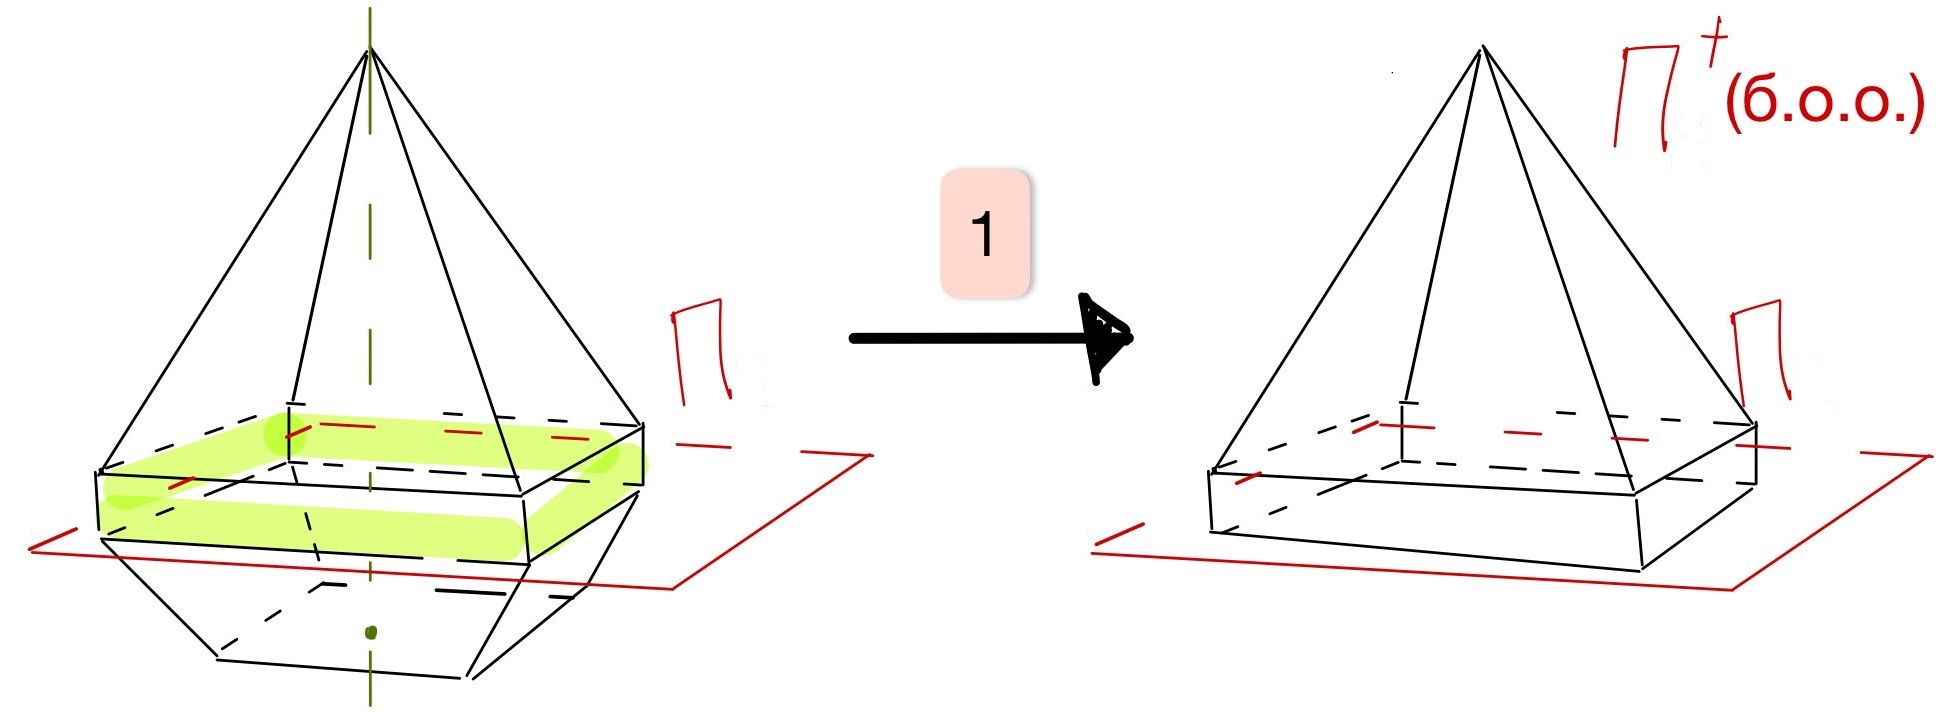
\includegraphics[scale=0.4]{PolyPlus.jpg}}
\end{figure}\vspace{1cm}

Будем пересекать $P^+$ плоскостями $\Pi_j$, параллельными $\Pi$. $CS_j(Cross Section)$ -- граница j-ого сечения, $j = 1, N_{cs}.$\newpage

\begin{figure}[h!]
\center{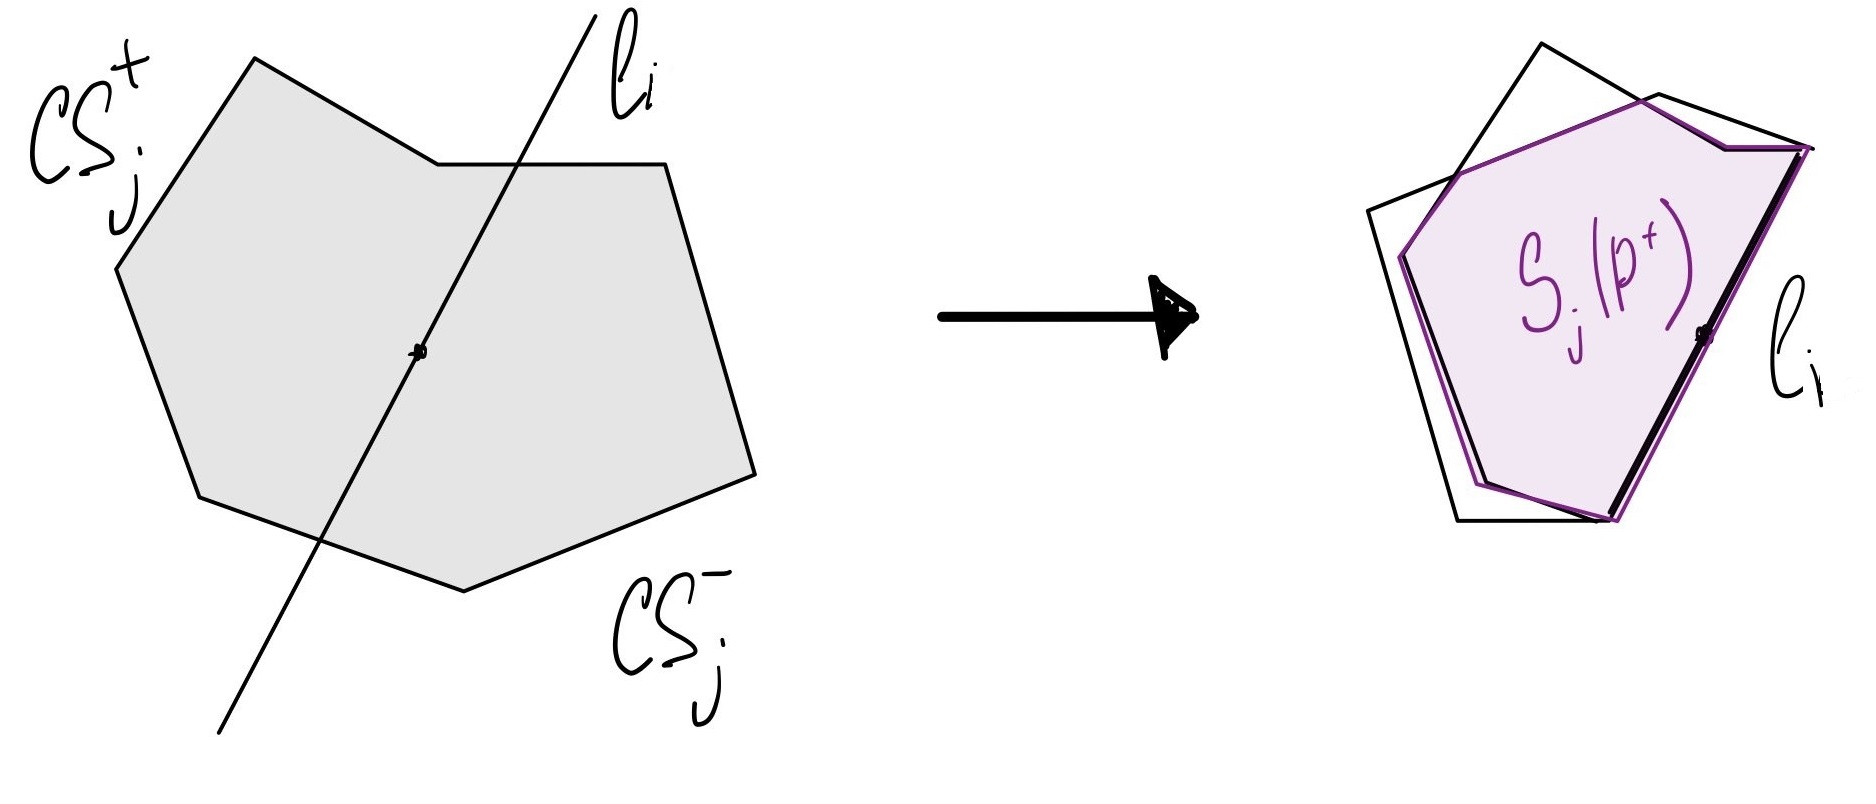
\includegraphics[scale=0.4]{Sym.jpg}}
\end{figure}

Введем меру симметричности $CS_j$. Для этого проведем $n$ прямых $l_i$ через центр многогранника P, спроецированного на $\Pi_j$, с шагом по углу $\dfrac{360}{n}$. $l_i$ делит $CS_j$ на две части: $CS_j^+, \; CS_j^-$. Отобразим $CS_j^-$ на $CS_j^+$ симметрично относительно $l_i$ (обозначение для отображенного $CS_j^-$ оставим тем же), найдем площадь пересечения и поделим ее на площадь $CS_j$ для нормировки:

$$\begin{gathered}
	S_j^i(P^+) := \dfrac{Area(CS_j^+ \cap CS_j^-)}{Area(CS_j)}.
\end{gathered}$$

Таким образом, набору R поставим в соответствие величину

$$\begin{gathered}
	Sym(R):= \sum\limits_{j = 1}^{N_{cs}}\sum\limits_{i = 1}^{n} S_j^i(P^+) + S_j^i(P^-).
\end{gathered}$$

\subsection*{\Large{Мера близости набора $R$ и аппроксимирующей ее цилиндрической поверхности Cyl.}}

R -- набор граней, Cyl -- аппроксимирующая его цилиндрическая поверхность. Для каждого множества граней R вычислим, насколько хорошо оно "ложится" на Cyl:

$$\begin{gathered}
	S_{Cyl}(R) := \dfrac{Area(R \cap Cyl)}{Area(R)}
\end{gathered}$$
\chapter{Рундист.}

\begin{definition}[Рундист]
	{\color{Black} \textbf{Рундист}} -- набор граней $R_0 = \{ Face_i\}_{i \in T_0} \in \{ R_i\},$ удовлетворяющий наибольшему числу следующих свойств:

	\begin{enumerate}
		\item $R_0$ имеет наибольшее число элементов среди остальных $R_i$:
		$$\begin{gathered}
		R_0 := \underset{R \in \{R_i\}}{argmax}(|R|)
		\end{gathered}$$

		\item полоса $R_0$ имеет наменьший размах среди остальных $R_i$:
		$$\begin{gathered}
		R_0 := \underset{R \in \{R_i\}}{argmin}(Amplitude(R))
		\end{gathered}$$

		\item угол между $l^{(up)}$ и $l^{(low)}$, соответствующий $R_0$, наименьший среди остальных $R_i$:
		$$\begin{gathered}
		R_0 := \underset{R \in \{R_i\}}{argmin}(sin(R))
		\end{gathered}$$

		\item через ось, перпендикулярную $\Pi(R_0)$ и проходящую через центр многогранника P, проходит наибольшее количество плоскостей симметрии относительно других $\Pi(R_i)$: 
		$$\begin{gathered}
		R_0 := \underset{R \in \{R_i\}}{argmax}(Sym(R))
		\end{gathered}$$

		\item набор $R_0$ лучше всех остальных $R_i$ аппроксимируется соответствующим цилиндром:
		$$\begin{gathered}
		R_0 := \underset{R \in \{R_i\}}{argmax}(S_{Cyl}(R))
		\end{gathered}$$

	\end{enumerate}
\end{definition}

\begin{remark}
	Константы, которые должны быть заданы:
	\begin{itemize}
		\item $N_{cs}$ -- количество сечений плоскостями для вычисления меры симметричности;
		\item n -- количество отражений для одного сечения при вычислении меры симметричности;
	\end{itemize}
\end{remark}

% \chapter{Используемые математические объекты}

\subsection*{Робастный метод наименьших квадратов.}

Рассмотрим пример. Для оценки p неизвестных параметров $\theta_1,\; \dots ,\theta_p$ используется n наблюдений $y_1,\; \dots,y_n$, причем они связаны между собой следующим неравенством $\mathbf{y}=X\mathbf{\theta}+\mathbf{u}$, где элементы матрицы X суть известные коэффициенты, а $\mathbf{u}$ - вектор независимых случайных величин, имеющих(приблизительно) одинаковые функции распределения.

Тогда решение сводится к решению следующей задачи: 
$$\begin{gathered}
	|\mathbf{y}-X\mathbf{\theta}|^2 \rightarrow \min
\end{gathered}$$

Если матрица X - матрица полного ранга p, то $\hat \theta={(X^{T}X)}^{-1}X^T\mathbf{y}$, а оценки $\hat y_i$ будут высиляться по следующей формуле:
$$\begin{gathered}
	\hat{\mathbf{y}} = H\mathbf{y},
\end{gathered}$$

\noindentгде $H=X{(X^{T}X)}^{-1}X^T$.

\begin{definition}
	H - матрица подгонки.
\end{definition}

Таким образом, получили значения $\hat y_i$ и остатки $r_i=y_i-\hat y_i$.

Пусть $s_i$ - некоторая оценка стандартной ошибки наблюдений $r_i$ю

Метрически винзоризуем наблюдения $y_i$, заменяя их псевдонаблюдениями ${y_i}^{\ast}$:


${y_i}^{\ast}=
\left{
y_i\,,   \;   \;\; |r_i| \le cs_i \\
\hat y_i - cs_i\,, \;\; r_i<-cs_i \\
\hat y_i + cs_i\,, \;\; r_i>cs_i
\right.$



% \cleardoublepage
\phantomsection
\addcontentsline{toc}{chapter}{Список используемой литературы}
\begin{thebibliography}{}
	\bibitem{0}
		Wiley Series in Probability and Statistics Established by Walter A. Shewhart and Samuel S. Wilks
\end{thebibliography}

\end{document}
